% 李奇中文简历 - 基于Clean CV模板
% 支持中文显示,清华紫色主题
% 
% 使用XeLaTeX编译以获得最佳中文显示效果
%
\documentclass[oneside]{article}

\usepackage{wallpaper}
\usepackage{geometry}
\usepackage[
    unicode=true,
    bookmarks=true,
    bookmarksnumbered=false,
    bookmarksopen=true,
    bookmarksopenlevel=1,
    breaklinks=false,
    pdfborder={0 0 0},
    backref=false,
    colorlinks=false
    ]{hyperref}
\usepackage{lastpage}
\usepackage{hyphenat}
\usepackage{hyphsubst}
\usepackage{tabularx}
\usepackage{moresize}
\usepackage[document]{ragged2e}

% 中文支持 - 使用系统可用字体
\usepackage{xeCJK}

% 使用系统可用的中文字体,最简配置避免字体不存在错误
% \setCJKmainfont{Noto Sans CJK SC}
% \setCJKsansfont{Noto Sans CJK SC}
% \setCJKmonofont{Noto Sans Mono CJK SC}

% xeCJK基础配置,避免复杂特性冲突
\xeCJKsetup{
  CJKmath=true,
  CheckSingle=true,
  PlainEquation=true
}

\usepackage[scaled]{helvet}
\usepackage{fontawesome5}
\usepackage[defaultfam,tabular,oldstyle]{montserrat}
\usepackage[T1]{fontenc}
\renewcommand*\oldstylenums[1]{{\fontfamily{Montserrat-TOsF}\selectfont #1}}

\usepackage{titlesec}
\usepackage{xcolor}
\usepackage{graphicx}
\usepackage{tikz}

\setlength{\parindent}{0pt}
\titleformat{\section}{\normalfont}{}{0pt}{}

\renewcommand{\arraystretch}{1.4}

\setlength\fboxrule{0pt}
\setlength\fboxsep{12pt}

\titlespacing{\section}{0pt}{1.5ex plus .1ex minus .2ex}{1pc}

\newcolumntype{Y}{>{\RaggedRight\arraybackslash}X}

% PDF元信息
\hypersetup{
    pdftitle={李奇 - 中文简历},
    pdfauthor={李奇},
    pdfsubject={学术简历}
}

% 页面设置
\geometry{
    a4paper,
    left=0pt,
    right=0pt,
    top=0pt,
    bottom=0pt,
    nohead,
    nomarginpar
}

% 颜色配置 - 清华紫色主题
\definecolor{sidebg}{RGB}{102, 45, 145}  % 清华紫 #662D91
\definecolor{mainbg}{RGB}{255, 255, 255}  % 纯白色
\definecolor{maintext}{RGB}{51, 51, 51}   % 深灰色文字
\definecolor{sidetext}{RGB}{255, 255, 255} % 侧边栏白色文字

\pagecolor{mainbg}

\begin{document}
\setlength{\topskip}{0pt}\setlength{\footskip}{0pt}%
\fcolorbox{red}{sidebg}{%
    \begin{minipage}[t][\textheight-2\fboxsep-2\fboxrule][t]{\dimexpr0.40\textwidth-2\fboxrule-2\fboxsep\relax}
        \color{sidetext}
        %%%%%%%%%%%%%%%%%%%%%%%%%%%%%%%%%%%%%%%%%%%%%%%%%%%%
        % 姓名和基本信息
        {\bfseries\scshape\HUGE 李} \\
        {\bfseries\scshape\Huge 奇} \quad {\normalfont\Large Qi Li}
        \vspace{.3cm} \\
        清华大学机械工程博士研究生 \\
        智能监测诊断技术 \\
        \textbf{总被引用:500+}
        \\
        % 头像
        \IfFileExists{../images/LQ.png}{
        \begin{center}
            \begin{tikzpicture}
            \clip (0,0) circle (3cm) node[anchor=center] {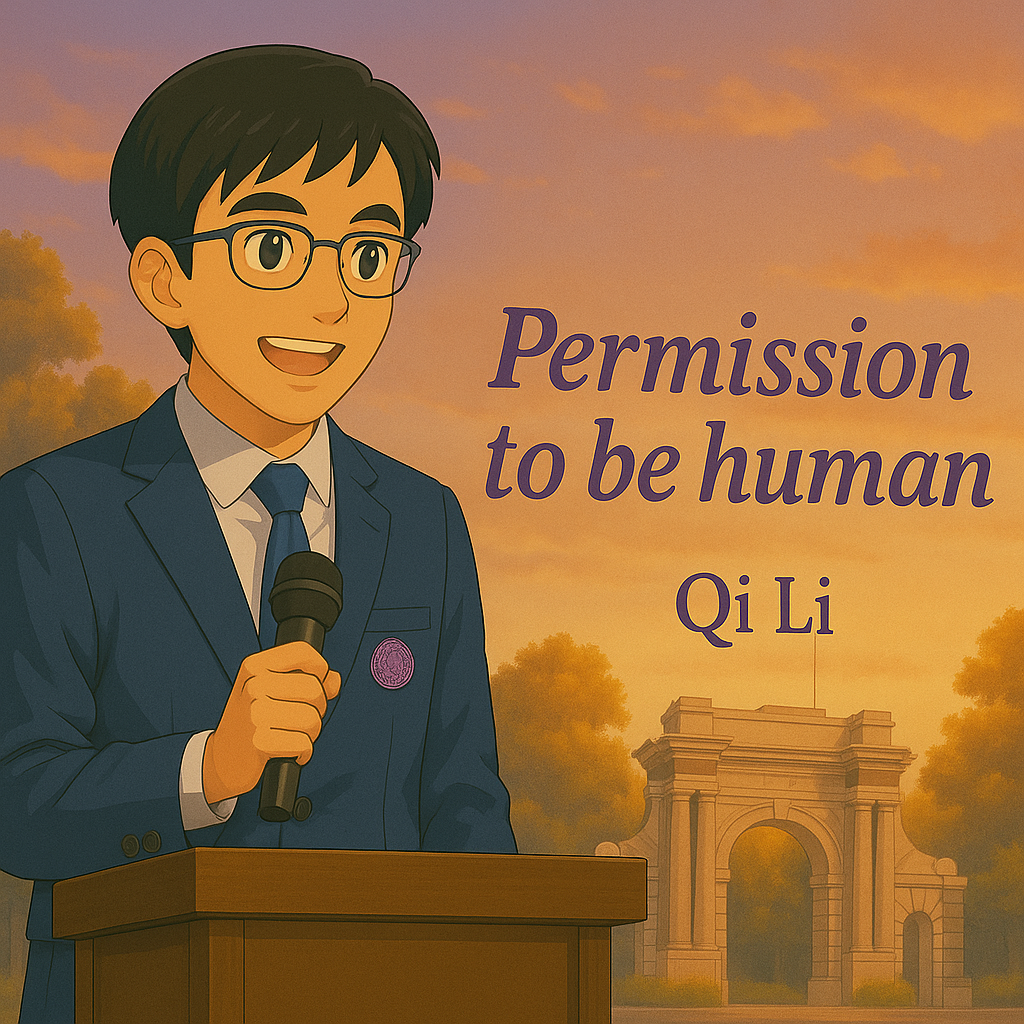
\includegraphics[width=6cm]{../images/LQ.png}}; 
            \end{tikzpicture}
        \end{center}
        }{}
        \vspace{.3cm}
        %%%%%%%%%%%%%%%%%%%%%%%%%%%%%%%%%%%%%%%%%%%%%%%%%%%%
        % 个人基本信息
        \phantomsection{}
        \addcontentsline{toc}{section}{个人信息}
        \section*{\large 个人信息}
        \begin{tabularx}{\textwidth}{cY}
            \faBirthdayCake{} & 1997年7月 \\
            \faFlag{}       & 汉族,浙江温州 \\
            \faUserTie{}    & 中共党员 \\
            \faPhone{}      & 18896782803 \\
            \faEnvelope{}   & \href{mailto:liq22@tsinghua.org.cn}{liq22@tsinghua.org.cn} \\
            \faGlobe{}      & \href{https://liq22.github.io/}{liq22.github.io} \\
            \faIdCard{}     & ORCID: 0000-0001-7105-2818 \\
        \end{tabularx}
        \vspace{.3cm} \\
        \rule{\linewidth}{0.4pt} \\
        %%%%%%%%%%%%%%%%%%%%%%%%%%%%%%%%%%%%%%%%%%%%%%%%%%%%%%%%%
        % 研究领域
        \phantomsection{}
        \addcontentsline{toc}{section}{研究领域}
        \section*{\large 研究领域}
        \begin{tabular}{cl}
            \faBrain{}      & 可信人工智能 \\
            \faCogs{}       & 基础模型 \\
            \faTools{}      & 智能监测诊断技术 \\
        \end{tabular}
        \vspace{10pt} \\
        \rule{\linewidth}{0.4pt} \\
        %%%%%%%%%%%%%%%%%%%%%%%%%%%%%%%%%%%%%%%%%%%%%%%%%%%%%%%%%%%%
        % 核心技能
        \phantomsection{}
        \addcontentsline{toc}{section}{核心技能}
        \section*{\large 核心技能}
        \begin{tabularx}{\textwidth}{cY}
            \faCode{}        & Python, MATLAB, PyTorch \\
            \faPen*{}        & TensorFlow, Scikit-learn \\
            \faFont{}        & LaTeX, 英文学术写作 \\
            \faLanguage{}    & 中文(母语), 英文(优秀) \\
            \faDesktop{}     & Linux, Windows, HPC集群 \\
            \faLaptopCode{}  & Jupyter, VS Code, PyCharm \\
        \end{tabularx}
        \vspace{1pt} \\
        \rule{\linewidth}{0.4pt}
        %%%%%%%%%%%%%%%%%%%%%%%%%%%%%%%%%%%%%%%%%%%%%%%%%%%%%%%%%%%%%%%%
        % 主要荣誉
        \phantomsection{}
        \addcontentsline{toc}{section}{主要荣誉}
        \section*{\large 主要荣誉}
        \begin{tabularx}{\textwidth}{cY}
            2024 & 首批科协青年托举人才(博士) \\
            2024 & 振动工程协会科学技术二等奖 \\
            2023 & 清华大学社会实践奖学金 \\
            2022 & 清华大学未来学者奖学金 \\
            2021 & 国家奖学金 \\
            2020 & 国家奖学金 \\
        \end{tabularx}
        \vspace{.3cm}
        \vfill
    \end{minipage}
}
\hfill
\fcolorbox{red}{mainbg}{%
    \begin{minipage}[t][\dimexpr\textheight-2\fboxrule-2\fboxsep\relax][t]{\dimexpr0.6\textwidth-2\fboxrule-2\fboxsep\relax}
        \color{maintext}
        %%%%%%%%%%%%%%%%%%%%%%%%%%%%%%%%%%%%%%%%%%%%%%%%%%%%%%%%%%
        % 学习经历
        \phantomsection{}
        \addcontentsline{toc}{section}{学习经历}
        \section*{\scshape\Large 学习经历 \rule{\linewidth}{0.4pt}}
%
        {\large \textbf{清华大学}} \\ 
        {{\fontseries{medium}\selectfont 机械工程博士}} \\
        {\scshape\fontseries{light}\selectfont\footnotesize 2022年9月 \textendash{} 2026年6月} 
        \begin{itemize}
            \setlength{\itemsep}{-3pt}
            \item 导师:秦朝烨 教授
            \item 专业方向:智能监测诊断技术
            \item 学术成果:5篇代表性论文,500+总被引用
            \item 获奖情况:未来学者奖学金、青年托举人才
        \end{itemize}
%
        {\large \textbf{耶鲁大学}} \\
        {{\fontseries{medium}\selectfont 访问学者,数据科学与统计系}} \\
        {\scshape\fontseries{light}\selectfont\footnotesize 2025年4月 \textendash{} 2025年9月} 
        \begin{itemize}
            \setlength{\itemsep}{-3pt}
            \item 导师:Lu Lu 教授
            \item 研究方向:物理信息神经网络
            \item 基础模型研究
            \item 国际学术合作与交流
        \end{itemize}
%
        {\large \textbf{苏州大学}} \\
        {{\fontseries{medium}\selectfont 控制理论与控制工程硕士}} \\
        {\scshape\fontseries{light}\selectfont\footnotesize 2019年9月 \textendash{} 2022年6月} 
        \begin{itemize}
            \setlength{\itemsep}{-3pt}
            \item 导师:陈亮 教授、沈长青 教授
            \item 研究重点:故障诊断的域适应方法
            \item 荣誉:江苏省优秀毕业生、优秀学术硕士毕业论文
            \item 成果:3篇ESI高被引论文
        \end{itemize}
%
        {\large \textbf{苏州大学}}\\
        {{\fontseries{medium}\selectfont 电气工程及其自动化学士}}\\
        {\scshape\fontseries{light}\selectfont\footnotesize 2015年9月 \textendash{} 2019年6月} 
        \begin{itemize}
            \setlength{\itemsep}{-4pt}
            \item 荣誉:优秀毕业生
            \item 特殊经历:开学典礼新生代表发言
            \item 基础:电气系统与控制工程扎实基础
        \end{itemize}
%
        {\large \textbf{瑞安市第十中学}}\\
        {{\fontseries{medium}\selectfont 高中}}\\
        {\scshape\fontseries{light}\selectfont\footnotesize 2012年9月 \textendash{} 2015年6月} 
        % \\
        \vfill%
        {\hfill\small\fontseries{extralight}\selectfont 第 \thepage 页,共 \pageref{LastPage} 页\hfill}
    \end{minipage}
}%
\newpage
%%%%%%%%%%%%%%%%%%%%%%%%%%%%%%%%%
% 第二页
%%%%%%%%%%%%%%%%%%%%%%%%%%%%%%%%%
\fcolorbox{red}{mainbg}{%
    \begin{minipage}[t][\dimexpr\textheight-2\fboxrule-2\fboxsep\relax][t]{\dimexpr0.6\textwidth-2\fboxrule-2\fboxsep\relax}
        \color{maintext}
        % \vspace{.6cm}
        %%%%%%%%%%%%%%%%%%%%%%%%%%%%%%%%%%%%%%%%%%%%%%%%
        % 代表性学术论文
        \phantomsection
        \addcontentsline{toc}{section}{代表性论文}
        \section*{\scshape\Large 代表性学术论文 \rule{\linewidth}{0.4pt}}
        \begin{justify}
        \setlength{\parindent}{0pt}
        {\large \textbf{深度专家网络研究}} \\
        {\scshape\fontseries{light}\selectfont\footnotesize JMS 2024 \qquad IF: 12.2, 中科院一区TOP} \\
        \textbf{Q. Li}, Y. Liu, S. Sun, Z. Qin, and F. Chu, "Deep expert network: A unified method toward knowledge-informed fault diagnosis via fully interpretable neuro-symbolic AI," J. Manuf. Syst., vol. 77, pp. 652–661, Dec. 2024.\\[1ex]

        {\large \textbf{透明算子网络研究}} \\
        {\scshape\fontseries{light}\selectfont\footnotesize IEEE TII 2024 \qquad IF: 11.7, 中科院一区TOP} \\
        \textbf{Q. Li}, H. Li, W. Hu, S. Sun, Z. Qin, and F. Chu, "Transparent Operator Network: A Fully Interpretable Network Incorporating Learnable Wavelet Operator for Intelligent Fault Diagnosis," IEEE Trans. Ind. Inf., 2024. \\[1ex]

        {\large \textbf{跨域增强诊断方法}} \\
        {\scshape\fontseries{light}\selectfont\footnotesize RESS 2023 \qquad IF: 9.4, ESI高被引, 被引51次} \\
        \textbf{Q. Li}, L. Chen, L. Kong, D. Wang, M. Xia, and C. Shen, "Cross-domain augmentation diagnosis: An adversarial domain-augmented generalization method for fault diagnosis under unseen working conditions," Reliab Eng Syst Saf, vol. 234, 2023. \\[1ex]
        
        {\large \textbf{对抗域不变泛化框架}} \\
        {\scshape\fontseries{light}\selectfont\footnotesize IEEE TII 2022 \qquad IF: 11.7, ESI高被引, 被引135次} \\
        L. Chen (导师), \textbf{Q. Li}, C. Shen et al. "Adversarial domain-invariant generalization: a generic domain-regressive framework for bearing fault diagnosis under unseen conditions," IEEE Trans. Ind. Informatics, 2021. \\[1ex]

        {\large \textbf{知识映射对抗域适应}} \\
        {\scshape\fontseries{light}\selectfont\footnotesize MSSP 2021 \qquad IF: 8.6, ESI高被引, 被引130次} \\
        \textbf{Q. Li}, C. Shen, L. Chen, et al. "Knowledge mapping-based adversarial domain adaptation: A novel fault diagnosis method with high generalizability under variable working conditions," Mech. Syst. Signal Process., vol. 147, 2021. \\[1ex]
        \end{justify}
        \vfill%
        {\hfill\small\fontseries{extralight}\selectfont 第 \thepage 页,共 \pageref{LastPage} 页\hfill}
    \end{minipage}
}
\hfill%
\fcolorbox{red}{sidebg}{%
    \begin{minipage}[t][\dimexpr\textheight-2\fboxrule-2\fboxsep\relax][t]{\dimexpr0.4\textwidth-2\fboxrule-2\fboxsep\relax}
        \color{sidetext}
        % \vspace{.5cm}
        %%%%%%%%%%%%%%%%%%%%%%%%%%%%%%%%%%%%%%%%%%%%%%%%%%%%%%%%
        % 第二页侧栏 - 姓名重复
        {\bfseries\scshape\HUGE 李} \\
        {\bfseries\scshape\Huge 奇} \quad {\normalfont\Large Qi Li}
        \vspace{.3cm} \\
        %%%%%%%%%%%%%%%%%%%%%%%%%%%%%%%%%%%%%%%%%%%%%%%%%%%%%%%%%%
        % 完整荣誉奖项
        \phantomsection
        \addcontentsline{toc}{section}{完整荣誉奖项}
        \section*{\large 完整荣誉奖项}
        \begin{tabularx}{\textwidth}{cY}
            2024 & 首批科协青年托举人才(博士) \\
            2024 & 振动工程协会科学技术二等奖 \\
            2023 & 清华大学社会实践奖学金 \\
            2023 & 江苏省优秀学术硕士毕业论文 \\
            2022 & 江苏省优秀毕业生 \\
            2022 & 清华大学未来学者奖学金 \\
            2021 & Best 3MT in UWA \\
            2021 & 江苏省优秀学生干部 \\
            2021 & 校优秀研究生 \\
            2021 & 国家奖学金 \\
            2020 & 国家奖学金 \\
        \end{tabularx}
        \vspace{.3cm}
        \\
        \rule{\linewidth}{0.4pt}
        \\
        %%%%%%%%%%%%%%%%%%%%%%%%%%%%%%%%%%%%%%%%%%%%%%%%%%%%%%%%%%%%
        % 学术服务
        \phantomsection
        \addcontentsline{toc}{section}{学术服务}
        \section*{\large 学术服务}
        \begin{tabularx}{\textwidth}{cY}
            \faJournalWhills{} & Information Fusion \\
            \faJournalWhills{} & IEEE TII, MSSP \\
            \faJournalWhills{} & Advanced Engineering Informatics \\
            \faJournalWhills{} & IEEE TIE, IEEE TIM \\
            \faJournalWhills{} & Measurement, MST \\
        \end{tabularx}
        \vspace{.3cm}
        \\
        \rule{\linewidth}{0.4pt}
        \\
        %%%%%%%%%%%%%%%%%%%%%%%%%%%%%%%%%%%%%%%%%%%%%%%%%%%%%%%%%%%%
        % 项目应用
        \phantomsection
        \addcontentsline{toc}{section}{项目应用}
        \section*{\large 项目应用}
        \begin{tabularx}{\textwidth}{cY}
            \faPlane{}      & 某型号飞机减振降噪分析 \\
            \faBolt{}       & 水电站智能运维技术 \\
            \faGithub{}     & PHMBench开源项目组负责人 \\
        \end{tabularx}
        \vspace{.3cm}
        \\
        \rule{\linewidth}{0.4pt}
        \\
        %%%%%%%%%%%%%%%%%%%%%%%%%%%%%%%%%%%%%%%%%%%%%%%%%%%%%%%%%%%%
        % 社会活动
        \phantomsection
        \addcontentsline{toc}{section}{社会活动}
        \section*{\large 社会活动}
        \begin{tabularx}{\textwidth}{cY}
            \faMicrophone{}  & 苏大开学典礼新生代表发言 \\
            \faUserTie{}     & 苏大机电学院研究生班长 \\
            \faHandsHelping{} & IFToMM会议志愿者 \\
        \end{tabularx}
        \vspace{.3cm}
        \\
        \rule{\linewidth}{0.4pt}
    \end{minipage}%
}%
\end{document}